% Created 2018-04-05 Thu 18:14
\documentclass[11pt]{article}\usepackage[]{graphicx}\usepackage[]{color}
%% maxwidth is the original width if it is less than linewidth
%% otherwise use linewidth (to make sure the graphics do not exceed the margin)
\makeatletter
\def\maxwidth{ %
  \ifdim\Gin@nat@width>\linewidth
    \linewidth
  \else
    \Gin@nat@width
  \fi
}
\makeatother

\definecolor{fgcolor}{rgb}{0.345, 0.345, 0.345}
\newcommand{\hlnum}[1]{\textcolor[rgb]{0.686,0.059,0.569}{#1}}%
\newcommand{\hlstr}[1]{\textcolor[rgb]{0.192,0.494,0.8}{#1}}%
\newcommand{\hlcom}[1]{\textcolor[rgb]{0.678,0.584,0.686}{\textit{#1}}}%
\newcommand{\hlopt}[1]{\textcolor[rgb]{0,0,0}{#1}}%
\newcommand{\hlstd}[1]{\textcolor[rgb]{0.345,0.345,0.345}{#1}}%
\newcommand{\hlkwa}[1]{\textcolor[rgb]{0.161,0.373,0.58}{\textbf{#1}}}%
\newcommand{\hlkwb}[1]{\textcolor[rgb]{0.69,0.353,0.396}{#1}}%
\newcommand{\hlkwc}[1]{\textcolor[rgb]{0.333,0.667,0.333}{#1}}%
\newcommand{\hlkwd}[1]{\textcolor[rgb]{0.737,0.353,0.396}{\textbf{#1}}}%
\let\hlipl\hlkwb

\usepackage{framed}
\makeatletter
\newenvironment{kframe}{%
 \def\at@end@of@kframe{}%
 \ifinner\ifhmode%
  \def\at@end@of@kframe{\end{minipage}}%
  \begin{minipage}{\columnwidth}%
 \fi\fi%
 \def\FrameCommand##1{\hskip\@totalleftmargin \hskip-\fboxsep
 \colorbox{shadecolor}{##1}\hskip-\fboxsep
     % There is no \\@totalrightmargin, so:
     \hskip-\linewidth \hskip-\@totalleftmargin \hskip\columnwidth}%
 \MakeFramed {\advance\hsize-\width
   \@totalleftmargin\z@ \linewidth\hsize
   \@setminipage}}%
 {\par\unskip\endMakeFramed%
 \at@end@of@kframe}
\makeatother

\definecolor{shadecolor}{rgb}{.97, .97, .97}
\definecolor{messagecolor}{rgb}{0, 0, 0}
\definecolor{warningcolor}{rgb}{1, 0, 1}
\definecolor{errorcolor}{rgb}{1, 0, 0}
\newenvironment{knitrout}{}{} % an empty environment to be redefined in TeX

\usepackage{alltt}\usepackage[]{graphicx}\usepackage[]{color}
%% maxwidth is the original width if it is less than linewidth
%% otherwise use linewidth (to make sure the graphics do not exceed the margin)

\usepackage{alltt}
\usepackage[utf8]{inputenc}
\usepackage[T1]{fontenc}
\usepackage{fixltx2e}
\usepackage{graphicx}
\usepackage{longtable}
\usepackage{float}
\usepackage{wrapfig}
\usepackage{rotating}
\usepackage[normalem]{ulem}
\usepackage{amsmath}
\usepackage{textcomp}
\usepackage{marvosym}
\usepackage{wasysym}
\usepackage{amssymb}
\usepackage{hyperref}
\tolerance=1000
\author{Timothy Schwieg}
\date{\today}
\title{Econometrics Homework 7}
\hypersetup{
  pdfkeywords={},
  pdfsubject={},
  pdfcreator={Emacs 25.1.1 (Org mode 8.2.10)}}
\IfFileExists{upquote.sty}{\usepackage{upquote}}{}
\IfFileExists{upquote.sty}{\usepackage{upquote}}{}
\begin{document}

\maketitle


\section{Question 1}
\label{sec-1}
\subsection{a}
\label{sec-1-1}
He could simply drive the same distance back and forth many times,
that is, drive the distance he walked n times in a row. There will
still be the same error on his starting odometer, and error on his
ending odometer, but since the value he is after is nd, his estimate
of d which is $\frac{nd}{n}$ has all the errors divided by n. By using
this strategy he may drive the error down to however small he wishes,
at the cost of the time spent driving that distance.

\subsection{b}
\label{sec-1-2}
Our measurement equation is given by:

\begin{align*}
S + nd + \xi_s &= E + \xi_e \\
nd &= E - S + \xi_e - \xi_s \\
d &= \frac{ E - S + \xi_e -\xi_s}{n}
\end{align*}
where $\xi_i \sim U(0,1)$

Our estimator $\hat{d}$ is given by $\frac{E - S}{n} = d + \frac{ \xi_s - \xi_e }{n}$

Since it is known that the mean-squared error is the bias squared plus
the variance, we need only calculate the bias and variance of $\hat{d}$.

\begin{align*} 
\mathbb{E}[ \hat{d} ] = d + \frac{ \mathbb{E}[\xi_s ] - \mathbb{E}[\xi_e ] }{n} = d \\
\mathbb{V} ( \hat{d} ) = \frac{1}{n^2} \mathbb{V}( \xi_s - \xi_e ) = \frac{1}{n^2} \left ( \mathbb{V}(\xi_s) + \mathbb{V}(\xi_e) \right ) \\
\frac{1}{n^2} \left ( \frac{1}{12} + \frac{1}{12} \right )  = \frac{ 1 }{6n^2}
\end{align*}

Thus the mean-squared error is given by: $\frac{1}{6n^2}$

\subsection{c}
\label{sec-1-3}
Following the notion on page 69 of Foundations of Empirical Intuition
by Harry Paarsch, it is known that the distribution of the difference
between two uniform random variables is given by:
\begin{align*}
  F_{\text{x}}(x) = \int_{\text{0}}^{\text{1}} \int_{\text{-1}}^{\text{x}} 1 dxdy = 
\begin{cases}
\frac{1}{2} + x + \frac{x^2}{2} \quad &-1 \leq x \leq 0 \\
\frac{1}{2} + x - \frac{x^2}{2} \quad &0 \leq x \leq 1
\end{cases}
\end{align*}

The density of the distribution is given by the derivative and is
thus:

$$f_x(x) = \begin{cases}
1 + x \quad &-1 \leq x \leq 0 \\
1 - x \quad &0 \leq x \leq 1
\end{cases}$$

Now for a series of random samples on n days, we can note that
\begin{align*}
S + d + \xi_s &= E + \xi_e \\
E - S &= d + \xi_s - \xi_e \\
\end{align*}

Thus the distribution of E-S is the difference of two uniforms,
shifted over to the right by d. Thus the distribution of the
difference is given by: 
\begin{align*}
F_Y(y) = P( d + \xi_s - \xi_e \leq y ) = P( \xi_s -\xi_e \leq y - d) \\
F_x( y - d ) = \begin{cases}
\frac{1}{2} + (y - d) + \frac{(y - d)^2}{2} \quad &d-1 \leq y \leq d \\
\frac{1}{2} + (y - d) - \frac{(y - d)^2}{2} \quad &d \leq x \leq d+1
\end{cases}
\end{align*}

and its density is given by:

\begin{align*}
f_x(x) = \begin{cases}
1 + y - d \quad &d-1 \leq y \leq d \\
1 - y - d \quad &d \leq y \leq d+1
\end{cases}
\end{align*}

The mean and variance of the measurement error are given by: 
\begin{align*}
\mathbb{E}[ \xi_s - \xi_e ] = .5 - .5 = 0 \\
\mathbb{V}( \xi_s - \xi_e ) = \mathbb{V}( \xi_s ) + \mathbb{V}( \xi_e ) = \frac{1}{6} \\
\end{align*}

\subsection{d}
\label{sec-1-4}

Since Y is given by the truth plus an error which has mean zero, its
bias will be zero, and by the linearity of expected value, any linear
combination of Y will be unbiased as well.

\begin{align*}
\mathbb{V}(\bar{Y}) = \mathbb{V}( \frac{1}{N} \sum_{n=1}^N y_n ) = \frac{1}{N^2} \sum_{n=1}^N \mathbb{V}( y_n ) = \frac{1}{6N}
\end{align*}

By applying the Lindinberg-Levy Central Limit theorem, we may note
that $\sqrt{N} \frac{ \bar{Y} - d }{ \sqrt{ \mathbb{V}(Y) } } \sim
N(0,1)$ Since $\bar{Y}$ is constructed by linear combinations of
uniform distributions, this will converge in distribution to the
normal quite quickly.

\subsection{e}
\label{sec-1-5}
Since the variance of the sample average is convergign on an order of
$O( \frac{1}{N} )$ it is converging relatively slower than part a which
is converging at a rate of $O( \frac{1}{N^2} )$. This means that you need
far fewer measurements, which makes intuitive sense, as the method in
part A only has the two errors which are uniform(0,1) present, while
the method suggested in the latter part has 2N errors which are all
uniform(0,1).

\section{Question 2}
\label{sec-2}
\begin{knitrout}
\definecolor{shadecolor}{rgb}{0.969, 0.969, 0.969}\color{fgcolor}\begin{kframe}
\begin{alltt}
\hlkwd{library}\hlstd{( gtools )}
\hlkwd{library}\hlstd{( ROCR )}

\hlkwd{set.seed}\hlstd{(} \hlnum{235711} \hlstd{)}

\hlstd{passFailData} \hlkwb{<-} \hlkwd{read.table}\hlstd{(} \hlstr{"PassFail.dat"}\hlstd{,} \hlkwc{header}\hlstd{=}\hlnum{FALSE} \hlstd{)}

\hlstd{nObs} \hlkwb{<-} \hlkwd{nrow}\hlstd{( passFailData )}

\hlcom{#There was some issues with sample() so we're doing it by hand}
\hlstd{order} \hlkwb{<-} \hlkwd{permute}\hlstd{(} \hlnum{1}\hlopt{:}\hlstd{nObs )}
\hlstd{trainSet} \hlkwb{<-} \hlstd{passFailData[order[}\hlnum{1}\hlopt{:}\hlkwd{floor}\hlstd{(nObs}\hlopt{*}\hlnum{.6}\hlstd{)],}\hlnum{1}\hlopt{:}\hlnum{7}\hlstd{]}
\hlstd{testSet} \hlkwb{<-} \hlstd{passFailData[order[(}\hlkwd{floor}\hlstd{(nObs}\hlopt{*}\hlnum{.6}\hlstd{)}\hlopt{+}\hlnum{1}\hlstd{)}\hlopt{:}\hlstd{nObs],}\hlnum{1}\hlopt{:}\hlnum{7}\hlstd{]}

\hlstd{model} \hlkwb{<-} \hlkwd{glm}\hlstd{(} \hlkwc{formula} \hlstd{= V1} \hlopt{~} \hlstd{.,} \hlkwc{family}\hlstd{=binomial,} \hlkwc{data}\hlstd{=trainSet )}

\hlstd{predLogit} \hlkwb{<-} \hlkwd{predict}\hlstd{( model ,} \hlkwc{newdata}\hlstd{=testSet[,}\hlopt{-}\hlnum{1}\hlstd{],}
                     \hlkwc{type}\hlstd{=}\hlstr{"response"}\hlstd{,} \hlkwc{se.fit} \hlstd{=} \hlnum{FALSE} \hlstd{)}

\hlcom{#Lets do a confustion matrix based on a tau of .5}
\hlstd{predictedValues} \hlkwb{<-} \hlkwd{floor}\hlstd{( predLogit} \hlopt{+} \hlnum{.5} \hlstd{)}

\hlstd{TP} \hlkwb{<-} \hlnum{0}
\hlstd{FP} \hlkwb{<-} \hlnum{0}
\hlstd{FN} \hlkwb{<-} \hlnum{0}
\hlstd{TN} \hlkwb{<-} \hlnum{0}

\hlkwa{for}\hlstd{( i} \hlkwa{in} \hlnum{1}\hlopt{:}\hlstd{(nObs}\hlopt{-}\hlkwd{floor}\hlstd{(}\hlnum{.6}\hlopt{*}\hlstd{nObs)) )\{}
    \hlkwa{if}\hlstd{( (predictedValues[i]} \hlopt{==} \hlstd{(testSet}\hlopt{$}\hlstd{V1)[i])} \hlopt{&&}
        \hlstd{(predictedValues[i]} \hlopt{==} \hlnum{1}\hlstd{) )\{}
        \hlstd{TP} \hlkwb{<-} \hlstd{TP} \hlopt{+} \hlnum{1}
    \hlstd{\}}
    \hlkwa{else if}\hlstd{( predictedValues[i]} \hlopt{!=} \hlstd{testSet}\hlopt{$}\hlstd{V1[i]} \hlopt{&&}
             \hlstd{predictedValues[i]} \hlopt{==} \hlnum{1} \hlstd{)\{}
        \hlstd{FP} \hlkwb{<-} \hlstd{FP} \hlopt{+} \hlnum{1}
    \hlstd{\}}
    \hlkwa{else if}\hlstd{( predictedValues[i]} \hlopt{==} \hlstd{testSet}\hlopt{$}\hlstd{V1[i] )\{}
        \hlstd{TN} \hlkwb{<-} \hlstd{TN} \hlopt{+} \hlnum{1}
    \hlstd{\}}
    \hlkwa{else} \hlstd{\{}
        \hlstd{FN} \hlkwb{<-} \hlstd{FN} \hlopt{+} \hlnum{1}
    \hlstd{\}}
\hlstd{\}}
\hlstd{TP}
\end{alltt}
\begin{verbatim}
## [1] 653
\end{verbatim}
\begin{alltt}
\hlstd{FP}
\end{alltt}
\begin{verbatim}
## [1] 396
\end{verbatim}
\begin{alltt}
\hlstd{FN}
\end{alltt}
\begin{verbatim}
## [1] 1022
\end{verbatim}
\begin{alltt}
\hlstd{TN}
\end{alltt}
\begin{verbatim}
## [1] 1929
\end{verbatim}
\end{kframe}
\end{knitrout}
From this data we can build a confusion matrix.
\begin{tabular}{|c|c|}\hline
  653&396\\\hline
  1022&1929\\\hline
\end{tabular}
\begin{knitrout}
\definecolor{shadecolor}{rgb}{0.969, 0.969, 0.969}\color{fgcolor}\begin{kframe}
\begin{alltt}
\hlstd{pred} \hlkwb{<-} \hlkwd{prediction}\hlstd{(predLogit, testSet}\hlopt{$}\hlstd{V1)}

\hlstd{auc} \hlkwb{<-} \hlkwd{performance}\hlstd{(pred,}\hlstr{"auc"}\hlstd{)}
\hlstd{auc}\hlopt{@}\hlkwc{y.values}
\end{alltt}
\begin{verbatim}
## [[1]]
## [1] 0.6654476
\end{verbatim}
\begin{alltt}
\hlstd{rocrCurve} \hlkwb{<-} \hlkwd{performance}\hlstd{( pred,}\hlstr{"tpr"}\hlstd{,}\hlstr{"fpr"} \hlstd{)}

\hlkwd{plot}\hlstd{( rocrCurve,} \hlkwc{xaxis}\hlstd{=}\hlstr{"tpr"}\hlstd{,} \hlkwc{yaxis}\hlstd{=}\hlstr{"fpr"}\hlstd{,}
     \hlkwc{main}\hlstd{=}\hlstr{"Logistic Regression"}\hlstd{,}
     \hlkwc{sub}\hlstd{=}\hlkwd{paste}\hlstd{(}\hlstr{"AUC: "}\hlstd{,} \hlkwd{toString}\hlstd{(auc}\hlopt{@}\hlkwc{y.values}\hlstd{[}\hlnum{1}\hlstd{]) ) )}
\end{alltt}
\end{kframe}
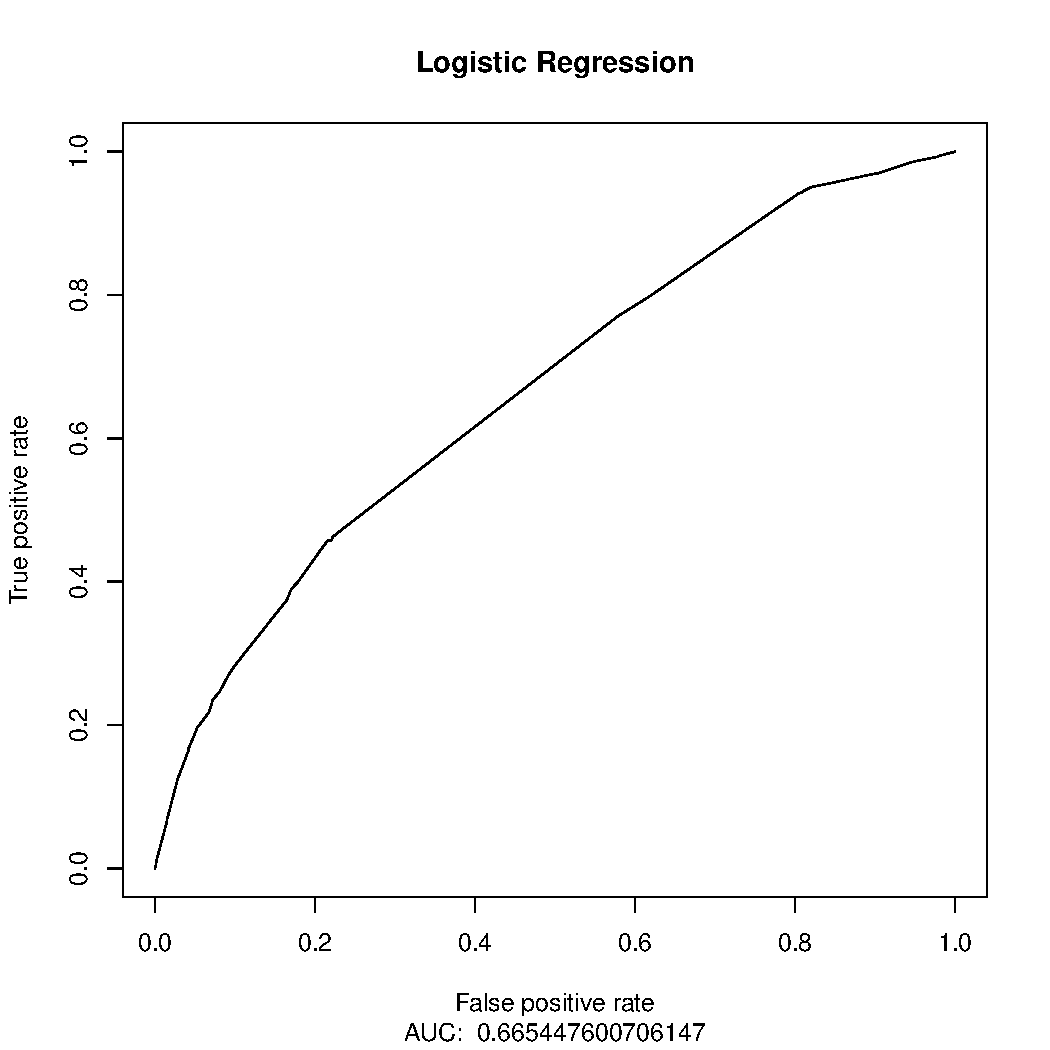
\includegraphics[width=\maxwidth]{figure/unnamed-chunk-1-1} 

\end{knitrout}


\end{document}
